\documentclass[10pt, a4paper]{article}

%import packages
\usepackage[pagestyles]{titlesec}
\usepackage{titlesec}
\usepackage{xcolor,colortbl}

%for lists and tables
\usepackage{enumitem}

%for section
\setcounter{secnumdepth}{3}
\setcounter{tocdepth}{3}

%for graphics
\usepackage{graphicx}

%package configurations
\pagestyle{empty}	
\renewcommand*\contentsname{\centering Table of Contents}
\titleformat{\section}{\centering\normalfont\Large\bfseries}{}{0pt}{}

%configures page number placement
\newpagestyle{main}{\setfoot{}{}{\thepage}}
\pagestyle{main}
\assignpagestyle{\chapter}{main}

%stuff from prof that handles formatting
\topmargin=0cm
\oddsidemargin=0cm
\textheight=22.0cm
\textwidth=16cm
\parindent=0cm
\parskip=0.15cm
\topskip=0truecm
\raggedbottom
\abovedisplayskip=3mm
\belowdisplayskip=3mm
\abovedisplayshortskip=0mm
\belowdisplayshortskip=2mm
\normalbaselineskip=12pt

\begin{document}


	
\hrulefill
\begin{flushright}
\textbf{Team PJ-b}
\end{flushright}
\hrulefill

\vspace*{0.5in}
\centerline{\bf\Large CODENAMES GAME}

%team members table
\vspace*{1.5in}


\begin{table}[htbp] 
\begin{center} 
	\begin{center} 
		Team Members\\
		
	\end{center} 
	\begin{tabular}{| c | c |} 
		\hline 
		Name & ID Number \\ 
		\hline\hline 
		Ashesh Patel & 40018519 \\ 
		Benjamin Th\'erien & 40034572\\ 
		Bilal Rana & 40013408 \\
		Christophe Savard & 40017812\\
		Daniel Thibault-Shea & 40073133\\ 
		Michael Wilgus & 29206388 \\ 
		Mordechai Zirkind & 27206151\\
		Rezza-Zairan Zaharin & 40003377 \\
		Shereece Victor & 40105094\\ 
		Steven Zanga & 40000797\\ 
		 
		\hline 
	\end{tabular} 
\end{center} 
\end{table} 

\newpage 
\tableofcontents 
\newpage 

\section{Project Analysis and Development Plan}

	\subsection{Introduction}
	
	 The purpose of this document is to detail the high-level requirements and features of the Codenames Game developed by team PJ-B. The Codenames Game is a game of 4 human and AI players. This project is an adaptation of the Codenames Game designed by Vlada Chv\'atil and published by Czech games.\\
	 \\
	 The specifics of how the Codenames Game fulfills these needs will be detailed in the use cases which more will be detailed in the upcoming design phase\\
	
	\subsection{Purpose}
	
	This document will describe the specifications entailed by the development of Codenames in compliance with the requirements of COMP 354. It will outline the high-level requirements encompassing user interfaces, product functions, user descriptions, assumptions and dependencies, constraints, specific requirements and an analysis model. The analysis model will hold use case diagrams, class diagrams, sequence diagrams and state transition diagrams.
	
	\subsection{Scope}
	
	%UPDATES ON FURTHER ITERATIONS
	This document only addresses the high level requirements of Codenames  that the design phase entails. The analysis model will contain UML diagrams used to serve multiple purposes. The Use case diagrams will give an overview of the functions of the project and how users will interact with it. The class diagrams will show the interactions between different objects in the game. \\
	

	\subsection{Definitions and Abbreviations}
	
		\subsubsection{Definitions}
	
		\textbf{Board} \\
		\\
		The main playing area will be composed of a 5 by 5 grid of words. Each cell of the grid are representative of Codenames of agents. Each cell in the grid will be defined in this document as a \textit{Card}.\\
	
		\textbf{Card} \\
		\\
		The card will hold two values indicative of it's state: hidden or revealed. In its hidden state, it will present a word taken from the game. In its revealed state, it can either be a blue or red team's \textit{Spy} card, a \textit{Civilian} card or the \textbf{Assassin} card.\\
		
		\textbf{Assassin} \\
		The Assassin is a card type that when revealed, it would cause the team that revealed it to lose.\\
		
		\textbf{Spy}\\
		\\
		The Spy is a card type that belongs to either the red or blue team. Once all spy cards of a team are revealed, the team wins.
		
		\textbf{Civilian}\\
		\\
		The Civilian is a card type that occupies leftover space on the board that is not occupied by \textit{Spy} cards or the \textit{Assassin} card. When revealed, it only skips the revealing team's turn. \\
	
	
	\subsection{Overview}
	
	The rest of this document outlines the problem description and the development plan. \\ 
	\\  
	The problem description will describe the game user's interfaces, product functions, user descriptions, assumptions and dependencies, constraints, specification requirements, and the analysis model. \\  
	
	\clearpage
	
\section{Problem Description}

	\subsection{Project Purpose, Scope, and Objectives}
	
	% Update for each iteration
	The objective of this project is to simulate a multi-user tabletop game named Codenames game by by Vlada Chv\'atil and published by Czech games. The rules of the game will intimately follow Vlada Chv\'atil with slight variations to accommodate the digital conversion. This project will be a multi-user game of up to four players; these players can be either human or computer players.\\
	
	By working on this project, Team PJ-b can experience the software engineering process entailing the difficulties in managing a group project.\\
	
	The project will be worked on over 3 iterations whereby they are the requirement phase, the design phase, and the test phase.
	
		\subsubsection{User interface}
		
		%Update by later iterations
		As this is the requirement phase, we are keeping the interface to a minimum design. They will not preface any visual grace but present the most useful information at the time. The visual representation of the game is as shown below:\\
		
		\begin{center}
			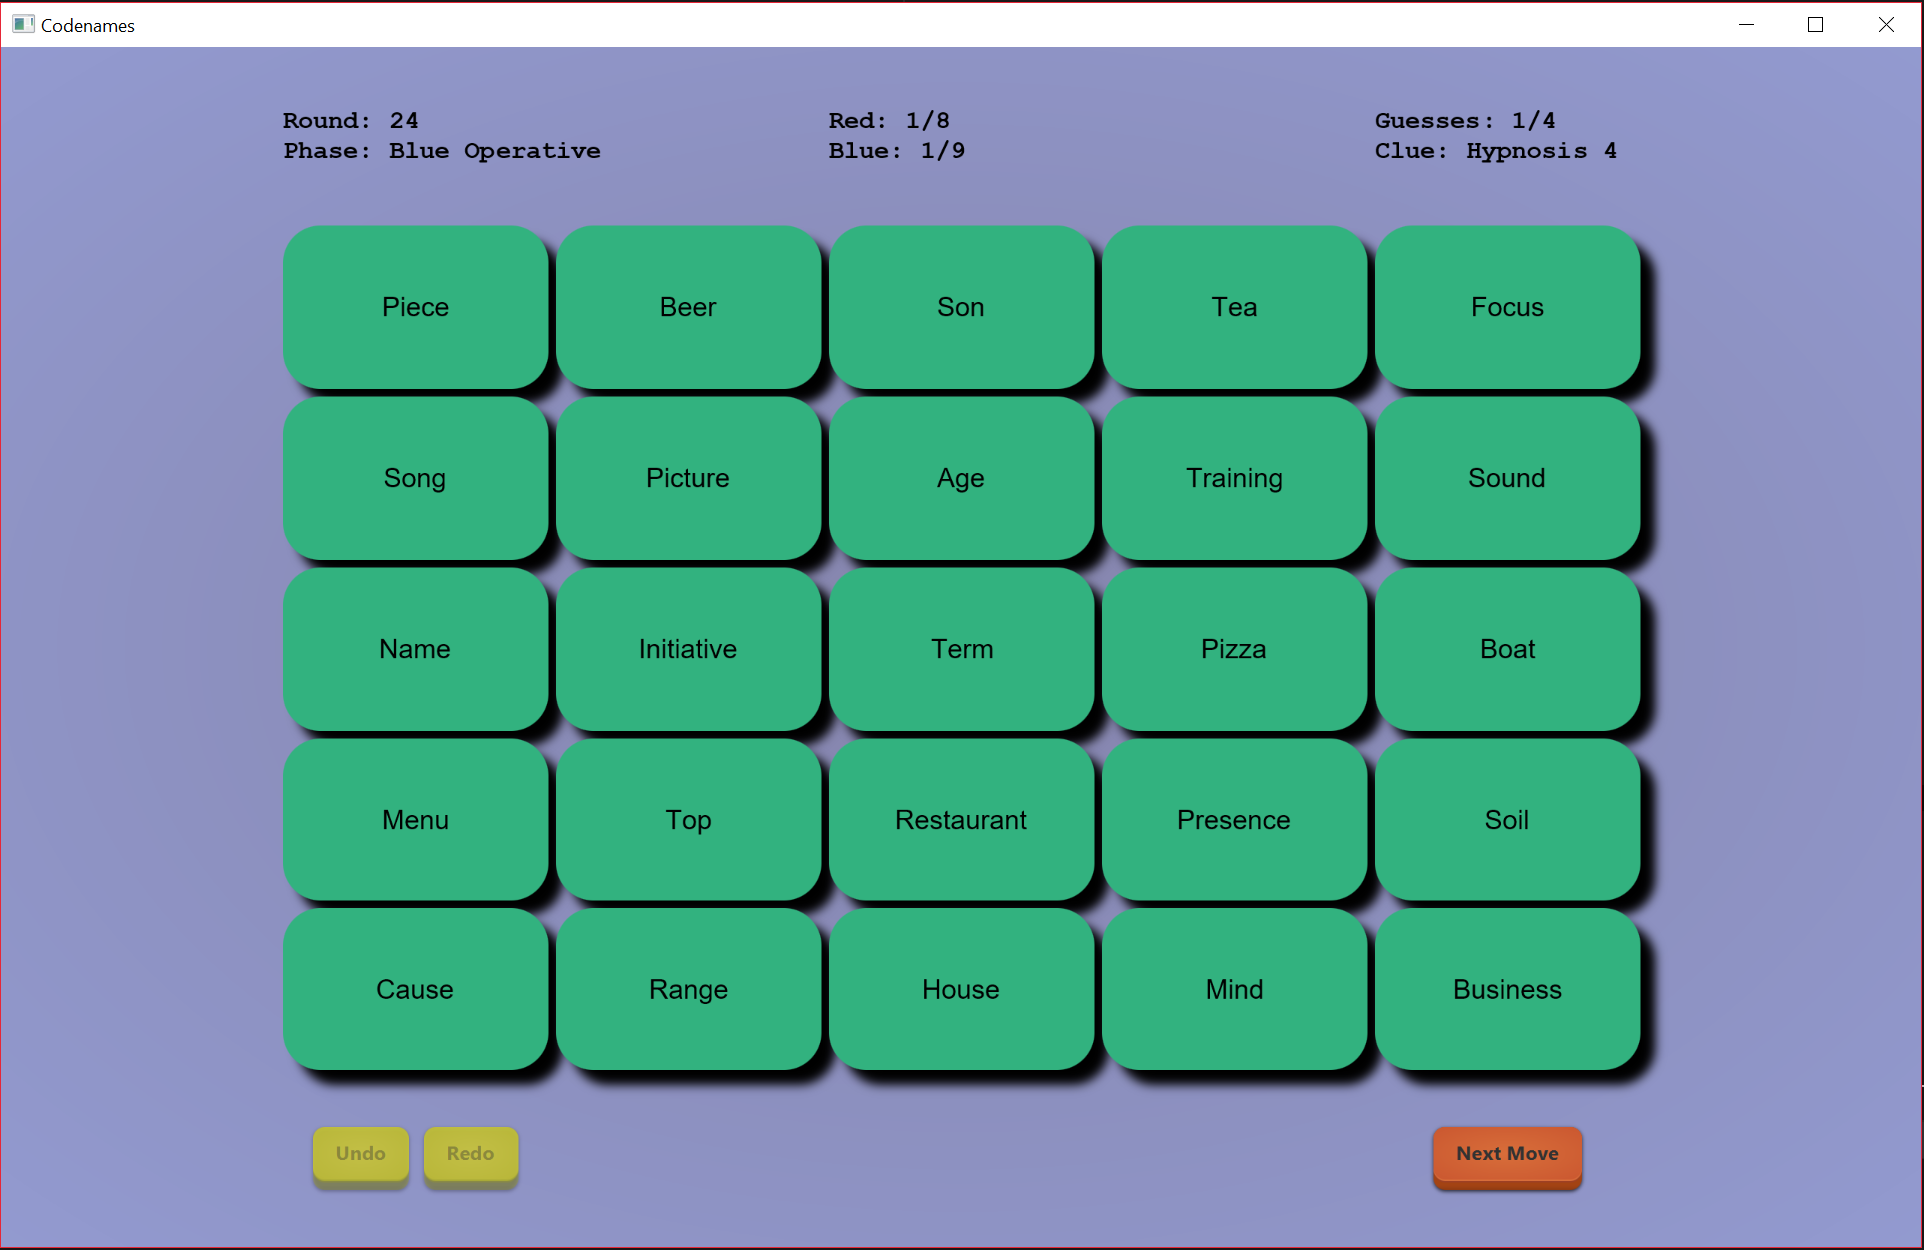
\includegraphics[scale=0.2]{game_interface.png}
		\end{center}
	
		\textbf{Board}\\
		\\
		The board is represented by a 5 by 5 set of cards, each possessing a word that when revealed, it will change in color to present what is the card type. When revealed, the card will be of a specific color to determine its value:  
		    \begin{itemize}
		        \item Red is a red spy.
		        \item Blue is a blue spy.
		        \item Black is \textit{the Assassin}.
		        \item Peach is a Civilian.
		    \end{itemize}
		    
	    \textbf{Round}\\
	    \\
	    On the top left, the "\textit{Round}" text represents the number of rounds that have passed in the game in accordance to the numerical value next to it.\\
	    
	    \textbf{Phase}\\
	    \\
	    On the top left, the "\textit{Phase}" text details the current player in action. This value would be either one of these at a time:
	        \begin{itemize}
	            \item Blue Spymaster
	            \item Blue Operative
	            \item Red Spymaster
	            \item Red Operative
	        \end{itemize}
	   
	   \textbf{Score-Keeping}\\
	   \\
	   In the middle top, Two sections with the text "\textit{Red}" and "\textit{Blue}" denotes the number of spies revealed for each team to the number of cards left to revealed. This is done in the format of:\\
	   
	   "Number of spies revealed / Total Number of spies"\\
	   
	   \textbf{Guesses}\\
	   \\
	    On the top right, the text "\textit{Guesses}" denotes the number of guesses left to be made by the \textit{Operative} given to by the \textit{Spymaster}. The value is formatted in: \\
	    
	   " Number of Guesses Left / Maximum Number of Guesses "\\
	   
	   \textbf{Clue}\\
	   \\
	   On the top right, the clue given by the \textit{Spymaster} will be displayed here.\\
	   
	   \textbf{Undo/Redo}\\
	   \\
	   On the bottom left, Two buttons of "\textit{Undo}" and "\textit{Redo}" functions as a point to click to control the turns elapsed. The \textit{Undo} button reverses a turn so long as it is made. The \textit{Redo} button replays a turn that was affected by \textit{Undo}.\\
	   
	   \textbf{Next Move}\\
	   \\
	   On the bottom right, the "\textit{Next Move}" button serves as a platform to click to progress the game forward by a turn.\\
	   
	   \clearpage
	
%	\subsection{Product Functions}
%	
%	Every function below has to support system  functions, such as a click of a button or revealing images when necessary. The following functions will be a part of the Codenames game.\\
%	
%		\subsubsection{Introduction}
%		
%		The user is first introduced to the game. Since human players are currently not being implemented into the game, only the "Start Game" button is visible. \\
%		
%		Input:
%		    \begin{itemize}
%		        \item The user clicks the "\textit{Start Game}" button.
%		    \end{itemize}
%	    
%		Action:
%		    \begin{itemize}
%		        \item 4 computer players are created: 2 for each team with each either being a \textit{Spymaster} or \textit{Operative}.
%		        \item 25 words are randomly picked from a database.
%		        \item The starting team is randomly picked.
%		    \end{itemize}
%		
%		Output:
%		    \begin{itemize}
%		        \item The teams are defined.
%		        \item A pool of words in use for the game are kept in an array.
%		        \item A turn order is decided.
%		    \end{itemize}
%		    
%		Validity Check:
%		    \begin{itemize}
%		        \item 
%		    \end{itemize}
%		
%		\subsubsection{Board}
%		
%		To be updated.\\
%		
%		\subsubsection{Game}
%		
%		There will be two teams of \textbf{red} and \textbf{blue}. Each team possesses a pair of players each playing either the role of Spymaster of Operative. Since each team follows the same path:\\
%		
%		\begin{itemize}
%			\item [--] Team \textit{Spymaster} reveals clue.
%			\item [--] Turn passes to Team's \textit{Operative}
%			\item [--] Team \textit{Operative} makes guesses based on clue given.
%			\item [--] Turn passes to opposing team's \textit{Spymaster}
%		\end{itemize}
%	
%		\textbf{Input:}\\
%		To be updated.\\
%		\\
%		\textbf{Action:}
%		To be updated.\\
%		\\
%		\textbf{Output:}\\
%		To be updated.\\
%		\\
%		\textbf{Validity Check:}\\
%		Sequence of the players is to be followed according to the order set earlier established. When a team finishes their turn, the next team's turn becomes active.\\
%		
	
	\subsection{Constraints}
	
	Assuming that a majority of player's PCs will run by the Windows OS, the project must be written in this platform that supports GUI.Thus, the decision has been made to use :
	\begin{itemize}
		\item[--] JAVA as the programming language.
		\item[--] SQLite as chosen for data storage.
		\item[--] JUnit for unit testing.
		\item[--] Eclipse as the integrated development environment(IDE).
	\end{itemize}
	
	\subsection{Analysis Models}
	
		\subsubsection{Use Case Diagrams}
		
		The following diagarams will help provide an overview of the functions in the game. They describe the action that a player can perform, as well as the interaction between some of the system functions which are not directly controlled by the player.\\
		
		These use case diagrams are included due to their importance in defining the user-to-software interactions, the requirements, and the scope of the system.\\
		
		The section below will detail the actors involved in the game: \\
		    
		    \textbf{User} \\
		    \\
		    The User represents the human player. For this iteration there is only one User. The User is able to control the chronological flow of the game via the use cases detailed below which are "\textit{Undo}", "\textit{Redo}", "\textit{Next Turn}", and "\textit{Start Game}".\\
		    
		    \textbf{Spymaster}\\
		    \\
		    The Spymaster is involved in the game by doling out clues. As there are only two teams, there will only be two Spymasters in the game. The Spymaster hands out clues via the "\textit{Reveal Clue}" use case detailed below.\\
		    
		    \textbf{Operative}\\
		    \\
		    The Operative is involved in the game by revealing cards in accordance to the clue and number of guesses given to by the Spymaster actor. As there are two teams, there will be only two Operatives in the game. The operative reveals cards through the use case "\textit{Reveal CARD}" use case as detailed below.\\
		    
		    \clearpage
		
			\paragraph{User Use Case}
			
			\begin{center}
				\includegraphics[scale=1.0]{"User UC".png}
			\end{center} 
			
			\paragraph{Spymaster and Operative Use Case}
			
			\begin{center}
				\includegraphics[scale=0.4]{"Spymaster & Operative UC".png}
			\end{center}
		
		\subsubsection{Use Cases Details}
		
			\paragraph{Use Case 1: Start Game }
			
			\begin{center}
				\begin{tabular}{ |c|p{10cm}| } 
					\hline
					Description & The Player commences the game  \\
					\hline 
					Actors & User \\
					\hline  
					Pre-Conditions & None \\
					\hline  
					Basic Path & 
						\begin{enumerate}
							\item The User clicks "Start Game".
							\item 4 Dummy players are generated and each are:
								\begin{itemize}
									\item Deposited into a team.
									\item Distributed a role.
								\end{itemize}
							\item The board is initialized.
							\item The card layout is randomized.
							\item The team turn order is randomized.
							\item The first turn order is given to the leading team's Spymaster.
						\end{enumerate}\\
					\hline
					Alternative Paths & None \\
					\hline
					Post-Conditions & 
						\begin{itemize}[noitemsep,topsep=0pt]
							\item The board has been initialized.
							\item 4 Dummy players are generated with their own team and role.
							\item The first player can play his/her turn.
						\end{itemize}\\
					\hline 
					Related Use Cases & \\
					\hline 
					Used Use Cases & None\\
					\hline 
					Extending Use Cases & None \\
					\hline 
				\end{tabular}
			\end{center}
		
			\newpage
			
			\paragraph{Use Case 2: Next Turn}
			
			\begin{center}
				\begin{tabular}{ |c|p{10cm}| } 
					\hline
					Description & The game moves forward a turn. \\
					\hline 
					Actors & User \\
					\hline  
					Pre-Conditions & \begin{itemize}[noitemsep,topsep=0pt]
						\item The Board is initialized.
						\item The game has not ended.
					\end{itemize} \\
					\hline  
					Basic Path & 
					\begin{enumerate}
						\item The user clicks the button, "Next Turn".
						\item The current acting player plays his/her turn.
						\item The turn passes to the next acting player.
					\end{enumerate}\\
					\hline
					Alternative Paths & None \\
					\hline
					Post-Conditions & A player has acted on his/her turn.\\
					\hline 
					Related Use Cases & \\
					\hline 
					Used Use Cases & None\\
					\hline 
					Extending Use Cases & None \\
					\hline 
				\end{tabular}
			\end{center}
		
			\paragraph{Use Case 3: Undo}
			
			\begin{center}
				\begin{tabular}{ |c|p{10cm}| } 
					\hline
					Description & The game reverses to a state before the current turn. \\
					\hline 
					Actors & User \\
					\hline  
					Pre-Conditions & \begin{itemize}[noitemsep,topsep=0pt]
						\item The user clicks the button,"Undo".
						\item The Board is initialized.
						\item At least a turn has been made.
					\end{itemize} \\
					\hline  
					Basic Path & 
					\begin{enumerate}
						\item The game reverses the actions done for the current turn.
						\item The turn is passed to the previously acting player.
					\end{enumerate}\\
					\hline
					Alternative Paths & None \\
					\hline
					Post-Conditions & A player has has his/her turn redacted.\\
					\hline 
					Related Use Cases & \\
					\hline 
					Used Use Cases & None\\
					\hline 
					Extending Use Cases & Redo \\
					\hline 
				\end{tabular}
			\end{center}
			
			\newpage
			
			\paragraph{Use Case 4: Redo}
			
			\begin{center}
				\begin{tabular}{ |c|p{10cm}| } 
					\hline
					Description & The game repeats action redacted by the "Undo" use case. \\
					\hline 
					Actors & User \\
					\hline  
					Pre-Conditions & \begin{itemize}[noitemsep,topsep=0pt]
						\item The user clicks the button "Redo"
						\item The Board is initialized.
						\item The "Undo" use case has been used at least once.
					\end{itemize} \\
					\hline  
					Basic Path & 
					\begin{enumerate}
						\item The game proceeds a turn with action undone by the use case "Undo".
						\item The turn is passed to the next acting player.
					\end{enumerate}\\
					\hline
					Alternative Paths & None \\
					\hline
					Post-Conditions & A player has has his/her turn redone.\\
					\hline 
					Related Use Cases & \\
					\hline 
					Used Use Cases & None\\
					\hline 
					Extending Use Cases & None \\
					\hline 
				\end{tabular}
			\end{center}
		
		\newpage
		
	\paragraph{Use Case 5: Reveal Clue}
		\begin{center}
		\begin{tabular}{ |c|p{10cm}| } 
			\hline
			Description & The Spymaster issues a clue \\ 
			\hline
			Actors & Spymaster \\
			\hline 
			Pre-Conditions & \begin{itemize}[noitemsep,topsep=0pt]
				\item The Board is initialized.
				\item The turn belongs to the Spymaster.
				\item The team Operative has not started his/her turn.
				\item There are still cards on the board to reveal.
			\end{itemize} \\
			\hline
			Basic Path & 
				\begin{enumerate}
					\item The Spymaster issues a clue with a number of guesses.
					\item The turn is passed to the team's Operative as detailed in the use case, "Reveal Card". 
				\end{enumerate} \\
			\hline 
			Alternative Paths & Alternative 1:
				\begin{enumerate}
					\item After step 1, if the clue not considered valid by the system (i.e. One or more words contains the clue word), the turn is passed to the Spymaster.
					\item The turn is also passed for the team Operative as detailed in the use case, "End Turn"
				\end{enumerate}\\
			\hline 
			Post-Conditions & 
				\begin{itemize}[noitemsep,topsep=0pt]
					\item A clue has been revealed
					\item The Spymaster’s turn has ended 
					\item The turn is passed to the team's Operative.
				\end{itemize} \\
			\hline 
			Related Use Cases & \\
			\hline 
			Used Use Cases & Reveal card, End Team's turn. \\
			\hline
			Extending Use Cases & None \\
			\hline
		\end{tabular}
	\end{center}

	\newpage
		
	\paragraph{Use Case 6: Reveal Card}
	\begin{center}
		\begin{tabular}{ |c|p{10cm}| } 
			\hline
			Description & The Operative reveals a card \\ 
			\hline
			Actors & Spymaster \\
			\hline 
			Pre-Conditions & \begin{itemize}[noitemsep,topsep=0pt]
				\item The Board is initialized.
				\item The team's Spymaster 
				\item The turn belongs to the Operative.
				\item The team Operative has not started his/her turn.
				\item There are still cards on the board to reveal.
				\item The number of guesses given by Spymaster is at least one.
			\end{itemize} \\
			\hline
			Basic Path & 
			\begin{enumerate}
				\item The Operative chooses to either:
				\begin{itemize}
					\item Continue to make guesses, proceed to step 2.
					\item End his/her turn, proceed to step 4.
				\end{itemize}
				\item The Operative reveals a card on the board.
				\item The number of guesses for the Operative is depleted by one.
				\item If there are still more than one guess left and there are cards to be revealed, repeat step 1.
				\item The turn is passed to the enemy Spymaster detailed in the use case, "Reveal clue". 
			\end{enumerate} \\
			\hline 
			Alternative Paths & 
			Alternative 1:
				\begin{itemize}[noitemsep,topsep=0pt]
					\item After step 2, If card revealed is an \textit{Enemy Spy} or \textit{Civillian}, the turn is passed to the enemy Spymaster detailed in the use case, "Reveal clue".
					\item If all of the enemy team's \textit{Spy} cards are revealed, the game ends with the enemy team winning.
				\end{itemize}
			Alternative 2:
				\begin{itemize}[noitemsep,topsep=0pt]
					\item After step 2, If card revealed is the \textit{Assassin} card, the game ends with the enemy team winning.
				\end{itemize}
			Alternative 3:
				\begin{itemize}[noitemsep,topsep=0pt]
					\item After step 2, If all of the Operative's \textit{Spy} cards are revealed, the game ends with the Operative's team winning.
				\end{itemize}\\
			\hline 
			Post-Conditions & 
			\begin{itemize}[noitemsep,topsep=0pt]
				\item A card is revealed on the board.
				\item The turn is passed to the enemy Spy.
			\end{itemize} \\
			\hline 
			Related Use Cases & \\
			\hline 
			Used Use Cases & Reveal Clue \\
			\hline
			Extending Use Cases & None \\
			\hline
		\end{tabular}
	\end{center}
	
	\newpage
	
		\subsubsection{Class Diagrams}
		a couple letters
			\paragraph{Full Class Diagram}
			a couple letters
			\paragraph{Simplified View}
			a couple letters
			\paragraph{Hierarchical View}
			a couple letters
	
\end{document}
